\documentclass{standalone}[9pt]
% main document, called main.tex
\usepackage{tikz}
\usetikzlibrary{external}
\tikzexternalize % activate!
\begin{document}

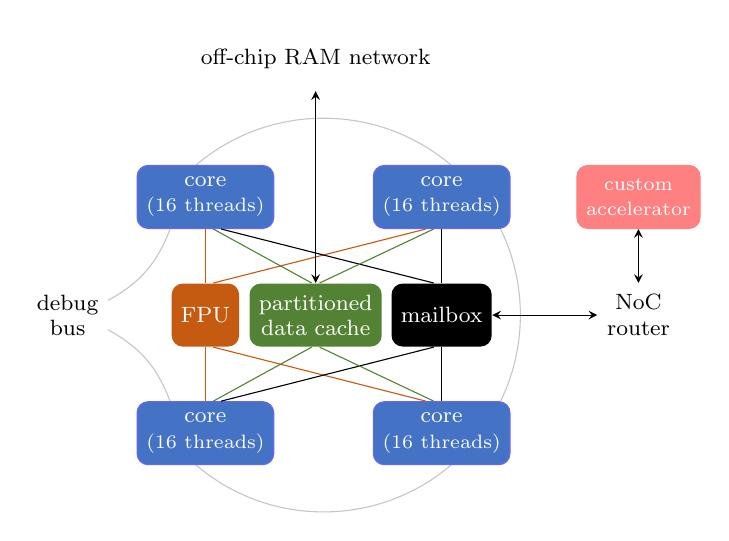
\begin{tikzpicture}
  [scale=.5,auto=left,every node/.style={rectangle,rounded
     corners,fill=myblue,text=white,minimum size=8mm},align=center]
  \definecolor{myblue}{RGB}{68,114,196}
  \definecolor{myorange}{RGB}{197,90,17}
  \definecolor{myorange}{RGB}{197,90,17}
  \definecolor{mygreen}{RGB}{84,130,53}

  \node[circle,draw=gray!45,fill=none,minimum width=5cm,minimum height=4.4cm] (tile) at (4,4) {};
  \node[minimum height=2.5cm,fill=white,text=gray] (blank) at (-1,4) {};
  \node[fill=white,text=black] (debug) at (-2.5,4)
    {\footnotesize{debug}\\[-1mm]
     \footnotesize{bus}};


  \node[draw=blue!60] (c1) at (1,1) {\footnotesize{core}\\[-1mm]\scriptsize{(16 threads)}};
  \node[draw=blue!60] (c2) at (7,1) {\footnotesize{core}\\[-1mm]\scriptsize{(16 threads)}};
  \node[draw=blue!60] (c3) at (1,7) {\footnotesize{core}\\[-1mm]\scriptsize{(16 threads)}};
  \node[draw=blue!60] (c4) at (7,7) {\footnotesize{core}\\[-1mm]\scriptsize{(16 threads)}};
  \node[fill=myorange] (fpu) at (1,4) {\footnotesize{FPU}};
  \node[fill=mygreen] (cache) at (3.8,4) {\footnotesize{partitioned}\\[-1mm]
                                        \footnotesize{data cache}};
  \node[fill=black] (mbox) at (7,4) {\footnotesize{mailbox}};

 
  \draw[color=gray!45,bend right=20] (debug) to
    ([xshift=-9mm,yshift=-8.2mm]c3);
  \draw[color=gray!45,bend left=20] (debug) to
    ([xshift=-9mm,yshift=8.2mm]c1);

  \draw[arrows=-,>=stealth,color=myorange] (c1.north) to (fpu.south);
  \draw[arrows=-,>=stealth,color=myorange] ([xshift=-4mm]c2.north) to
                                           ([xshift=2mm]fpu.south);
  \draw[arrows=-,>=stealth,color=myorange] (c3.south) to (fpu.north);
  \draw[arrows=-,>=stealth,color=myorange] ([xshift=-4mm]c4.south) to
                                           ([xshift=2mm]fpu.north);

  \draw[arrows=-,>=stealth,color=black] ([xshift=4mm]c1.north) to
                                        ([xshift=-2mm]mbox.south);
  \draw[arrows=-,>=stealth,color=black] (c2.north) to (mbox.south);
  \draw[arrows=-,>=stealth,color=black] ([xshift=4mm]c3.south) to
                                        ([xshift=-2mm]mbox.north);
  \draw[arrows=-,>=stealth,color=black] (c4.south) to (mbox.north);

  \draw[arrows=-,>=stealth,color=mygreen] ([xshift=2mm]c1.north) to
                                          ([xshift=-1mm]cache.south);
  \draw[arrows=-,>=stealth,color=mygreen] ([xshift=-2mm]c2.north) to
                                          ([xshift=1mm]cache.south);
  \draw[arrows=-,>=stealth,color=mygreen] ([xshift=2mm]c3.south) to
                                          ([xshift=-1mm]cache.north);
  \draw[arrows=-,>=stealth,color=mygreen] ([xshift=-2mm]c4.south) to
                                          ([xshift=1mm]cache.north);

  \node[draw=red!50, fill=red!50] (custom) at (12,7) {\scriptsize{custom}\\[-1mm]\scriptsize{accelerator}};

  \node[text=black,fill=none] (noc) at (12,4)
    {\footnotesize{NoC}\\[-1mm]
     \footnotesize{router}};

  \draw[arrows=<->,>=stealth] (custom) to (noc);

  \draw[arrows=<->,>=stealth] (mbox) to (noc);

  \node[text=black,fill=none] (noc) at (3.8,10.5)
    {\footnotesize{off-chip RAM network}};

  \draw[arrows=<->,>=stealth] (cache) to (noc);
\end{tikzpicture}

\end{document}
